\documentclass{parcfd}

\usepackage{graphicx}
\usepackage{subcaption}
\usepackage{amsmath}
\usepackage{amsfonts}
\usepackage{amssymb}
\usepackage{enumitem}

\graphicspath{{figures/}}

\title{REPLICATION STUDIES AND REPRODUCIBILITY CHECKLIST FOR COMPUTATIONAL FLUID DYNAMICS}

\author{Olivier MESNARD$^{*}$ and Lorena A. BARBA$^{*}$}

\heading{Lorena A. Barba and Olivier Mesnard}

\address{$^{*}$ Dept.\ of Mechanical \& Aerospace Engineering, George Washington University,
20052 Washington DC, USA\\
e-mail: labarba@gwu.edu, web page: http://lorenabarba.com}

\keywords{Reproducibility, Replicability, Immersed boundary method, containerization, Reproducibility checklist}

\abstract{We conducted replication of previously published studies to highlight sources of non-reproducibility in CFD. Our objective is to develop guidance on the computational artifacts and the level of detail needed for reproducibility and replication to be possible. We propose a reproducibility checklist tailored for CFD, which could be used by journals and conferences like ParCFD.}

\begin{document}
%\maketitle

\section{INTRODUCTION}

We rely on computer simulations and data models to create new knowledge.
But how much evidence do we need to provide to be confident of the new findings claimed in a publication or conference talk?
Published studies rarely come with the underlying software and computational steps that produced the results.
Software can have bugs and articles can have typos.
When researchers do not make their code and data available, there is little hope of knowing how data were processed to verify the results.

In 2019, the National Academies of Sciences, Engineering, and Medicine released a consensus report \cite{nasem_2019} with findings and recommendations to improve rigor and transparency in research.
The report also gives definitions, intended to apply across all fields of science:

\begin{description}
    \item[Reproducibility] is obtaining consistent results using the same input data; computational steps, methods, and code; and conditions of analysis.
    \item[Replicability] is obtaining consistent results across studies aimed at answering the same scientific question, each of which had obtained its own data. Two studies may be considered to have replicated if they obtain consistent results given the level of uncertainty inherent in the system under study.
\end{description}

We have already published on our efforts to replicate our own results and the many obstacles we faced \cite{mesnard_barba_2017}.
We now explore the effort it takes to replicate the computational results from other research groups.

Our objectives are (1) investigate causes of non-reproducibility in computational fluid dynamics applications, particularly in HPC situations; (2) conduct replication of previously published computational results, looking to identify sources of non-replicability; (3) develop guidance on what computational artifacts and what level of detail need to be shared for reproducibility and replication to be possible; (4) design workflows for computational research to guarantee, as much as possible, that findings are both reproducible and replicable.

\section{REPLICATION STUDIES}

We attempted to replicate two computational articles: one presents a new immersed boundary method, the other a study on the unsteady wake dynamics of pitching-rolling wings.
The computational code, input data, and conditions of analysis used to produce the published results are not available, thus we consider the studies to be not reproducible.
But, can we replicate the scientific findings? And can we do it in a reproducible way?

\subsection{Reproducible workflow}

Our open-source software, PetIBM, solves the incompressible Navier-Stokes equations via a projection method on structured Cartesian grids, with an immersed boundary method.
It uses PETSc to run in parallel, and AmgX to run on GPU devices.
We follow an open-source development model on GitHub.
PetIBM is licensed under BSD 3-clause, archived in Zenodo, and published in the Journal of Open Source Software \cite{chuang_et_al_2018}.

To capture the computational environment, we use container technologies.
Previously, we used Docker to achieve a reproducible workflow on Microsoft Azure \cite{mesnard_barba_2020} public cloud.
Now, we adopt a similar reproducible workflow but on a University-managed HPC cluster.
Docker is not available at most HPC centers for security concerns; the Docker daemon requires root privileges that users do not have on shared production clusters.
Instead, HPC centers can use the container technology of Singularity, which was designed from the ground up to prevent escalation of user privileges.
Singularity images used to produce our results are made publicly available on the registry SingularityHub.
Researchers interested in reproducing our results can pull these images to create a faithfully reproduced computational environment.

\subsection{First replication study}

Li \& co-authors \cite{li_et_al_2016} modified the immersed boundary projection method, decoupling the solution variables through an additional block-LU decomposition.
This results in a classical pressure Poisson system.

We implemented the algorithms presented by Li et al.\ in a PetIBM application, and made it open source.
Our replication study highlights differences in the numerical results when re-implementing the ``same'' algorithms (Figure \ref{fig:cylinder2dRe40:pressure_coefficient}).

\begin{figure}
    \centering
    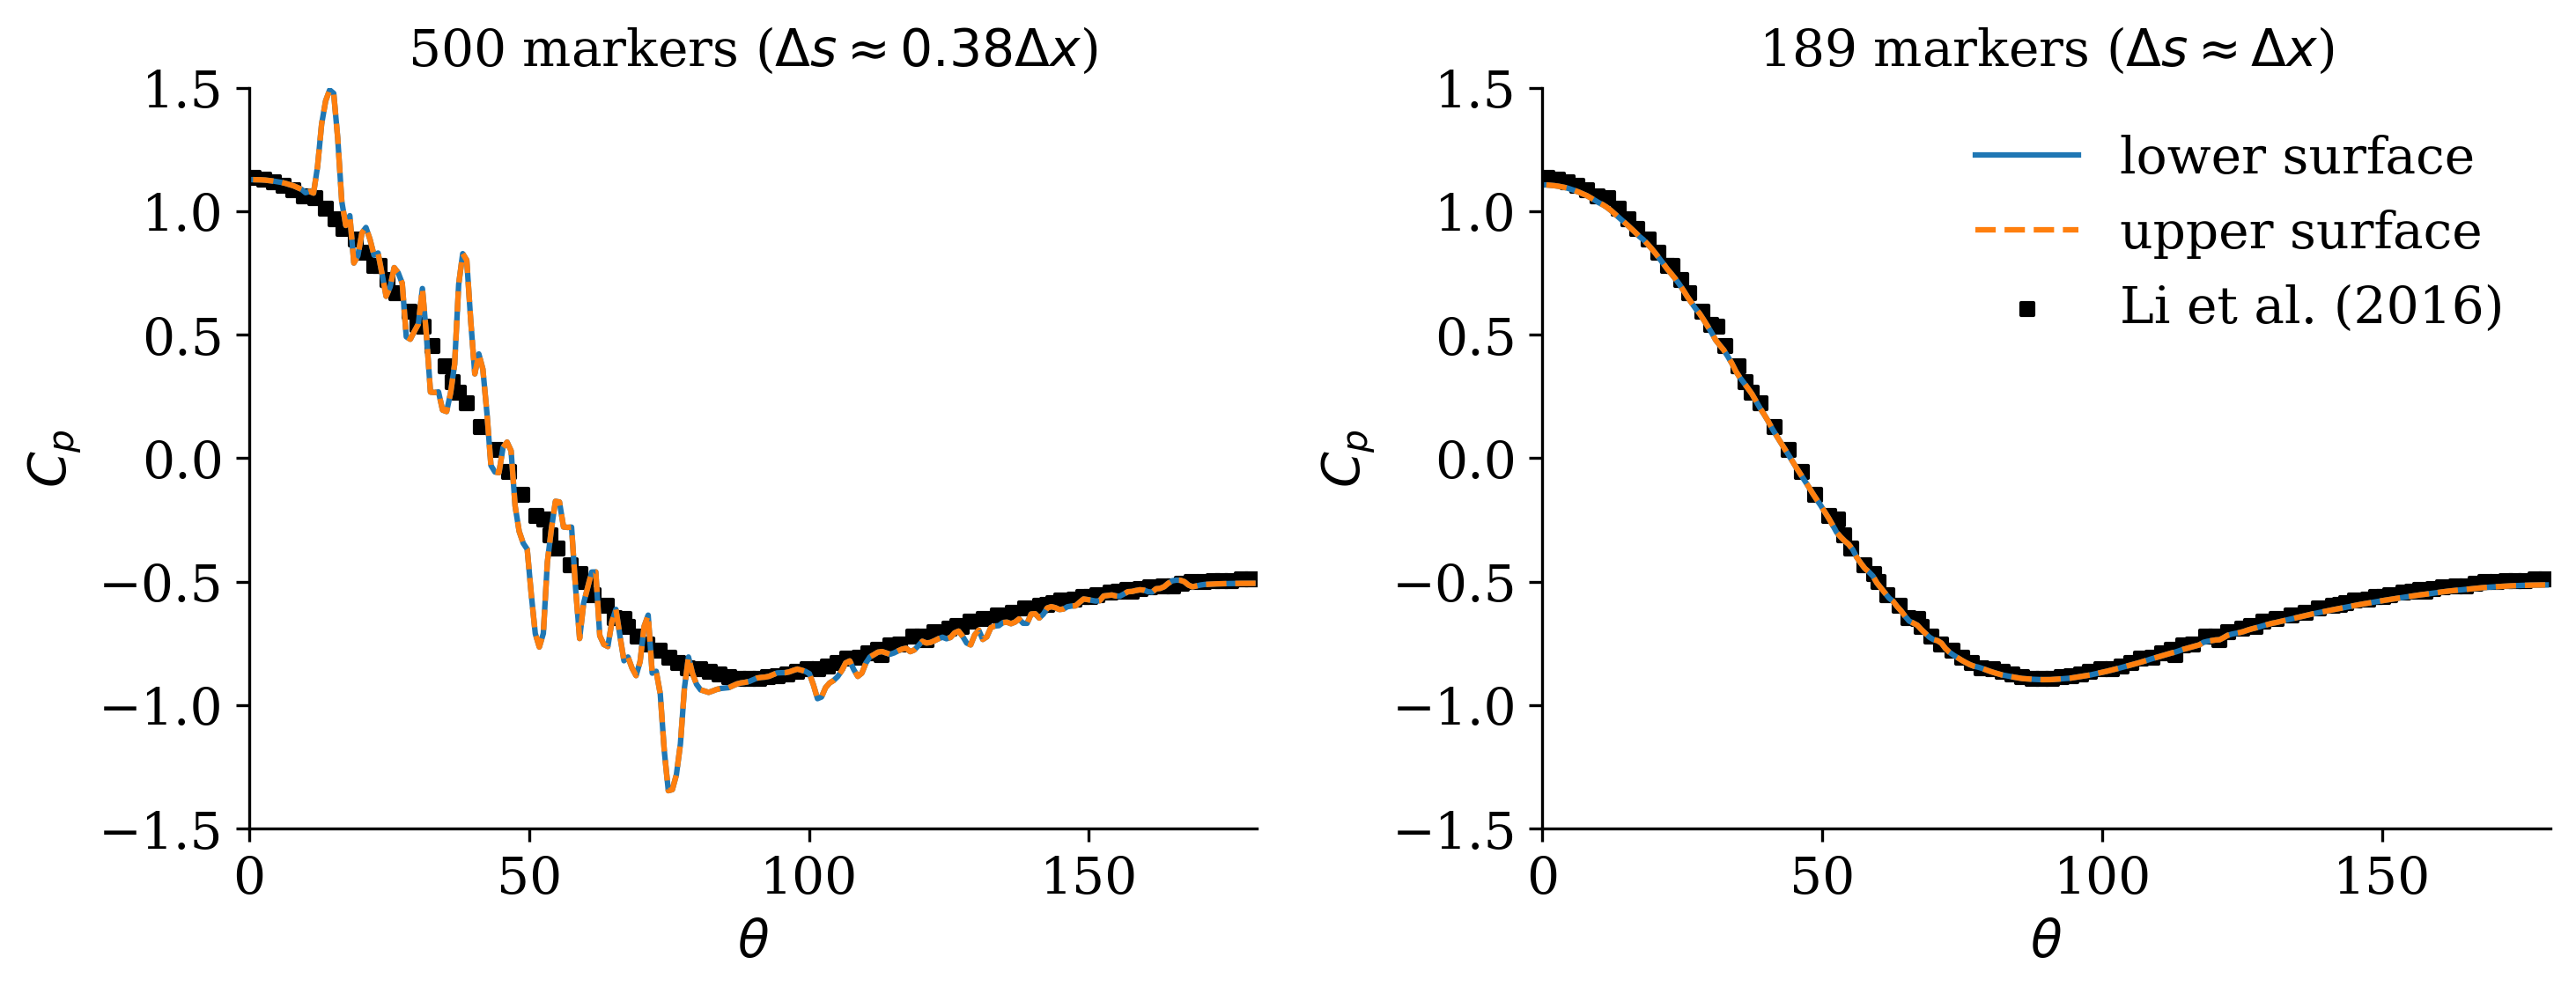
\includegraphics[width=0.8\linewidth]{cylinder2dRe40_pressure_coefficient.png}
    \caption{\small Distribution of the pressure coefficient along the surface of a stationary cylinder at Reynolds number $40$. With PetIBM, we used two different resolutions to discretize the immersed boundary: (left) $500$ equally spaced markers as in the original study \cite{li_et_al_2016} and (right) $189$ markers to maintain a similar resolution between the Lagrangian surface mesh and Eulerian grid.}
    \label{fig:cylinder2dRe40:pressure_coefficient}
\end{figure}

\subsection{Second replication study}

Li \& Dong \cite{li_dong_2016} conducted a parametric study of the rolling-pitching motion of a 3D elliptical plate, describing its wake topology and propulsive performance.
They used an in-house research code that implements a different immersed-boundary method (sharp-interface technique with a ghost-cell methodology) that those in PetIBM (diffused-interface method through regularized delta functions).

We have implemented the three-dimensional rolling and pitching kinematics (Figure \ref{fig:rollingpitching}) in a PetIBM application, and made it open source.
Our goal is to replicate the scientific findings with our code base and highlight possible differences in the results that may come from the use of different immersed-boundary techniques.

\begin{figure}
    \centering
    \begin{subfigure}{0.4\textwidth}
        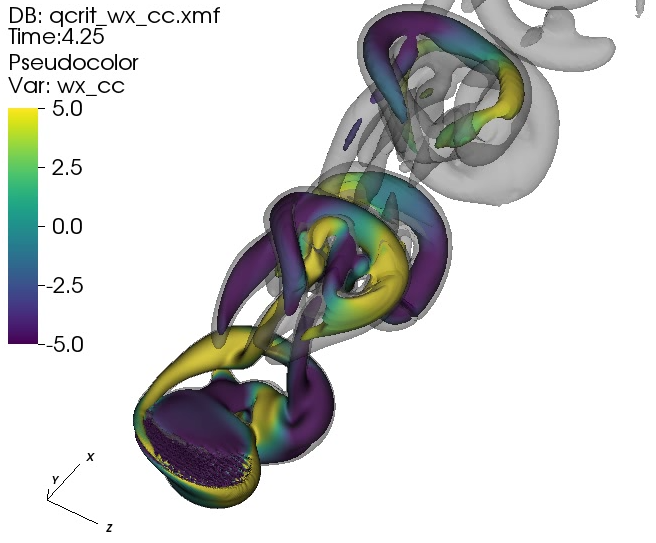
\includegraphics[width=\linewidth]{rollingpitching_perspective.png}
        \caption{}
        \label{fig:rollingpitching:perspective}
    \end{subfigure}
    \hspace*{1cm}
    \begin{minipage}{0.3\textwidth}
        \begin{subfigure}{\linewidth}
            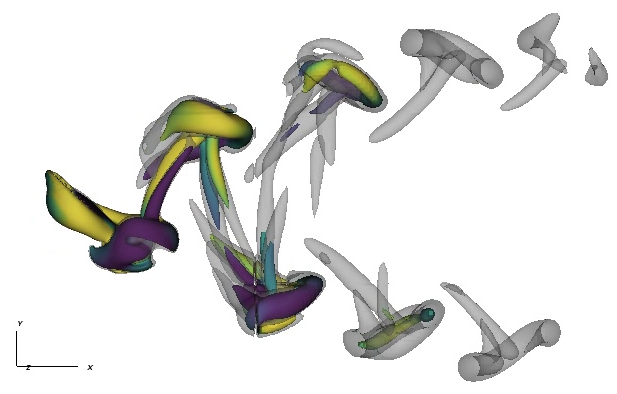
\includegraphics[width=\linewidth]{rollingpitching_side_view.png}
            \caption{}
            \label{fig:rollingpitching:side_view}
        \end{subfigure}
        \vspace*{0cm}
        \begin{subfigure}{\linewidth}
            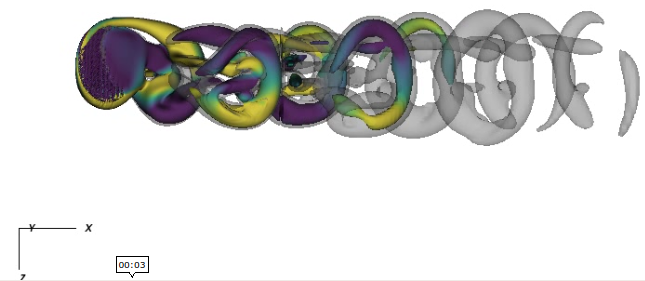
\includegraphics[width=\linewidth]{rollingpitching_top_view.png}
            \caption{}
            \label{fig:rollingpitching:top_view}
        \end{subfigure}
    \end{minipage}
    \caption{\small Wake topology of a pitching and rolling circular plate after four flapping cycles at Reynolds number $Re = 200$ and Strouhal number $St = 0.6$. Flow structures are visualized using the Q-criterion for $Q = 1$ (colored by the streamwise vorticity) and $Q = 6$ (gray). (a) Perspective view, (b) side view, (c) top view.}
    \label{fig:rollingpitching}
\end{figure}

\section{HOW ABOUT A REPRODUCIBILITY CHECKLIST FOR CFD?}

On the basis of these efforts, we are developing ``Reproducibility Checklists'' for adoption by journals wanting to improve the reproducibility of their articles, by incorporating this aspect in the peer-review criteria.
Other fields already started implementing such reproducibility checklists.
At the NeuroIPS-2019 conference, authors were asked to answer questions from a ``Machine Learning Reproducibility Checklist'' during submission.

Such reproducibility checklist for CFD might include these categories: Numerical analysis; Computational environment; Software management; Data management; Computational runtime.
We propose to order the items in the list in increasing levels of reproducibility, starting with the minimum requirements, acknowledging that some authors may not be able to comply with all of them.
For example, the ``Software Management'' category might ask if the following are satisfied:

\begin{small}
\begin{itemize}[noitemsep]
    \item[$\square$] the software is under version-control.
    \item[$\square$] the software is shared under an open-source license.
    \item[$\square$] the software version used in the manuscript is deposited in a data archival service (figshare, Zenodo, etc.).
    \item[$\square$] the code base is developed following a standard branching model, using an issue tracker, pull requests, code review.
    \item[$\square$] the software was reviewed and published in the Journal of Open Source Software
\end{itemize}
\end{small}

\begin{thebibliography}{99}
    \bibitem{nasem_2019} {National Academies of Sciences, Engineering, and Medecine.} \textit{Reproducibility and Replicability in Science.} Washington, DC: The National Academies Press (2019).
    \bibitem{mesnard_barba_2017} Mesnard, O. and Barba, L.A. Reproducible and replicable computational fluid dynamics: it's harder than you think. \textit{Computing in Science \& Engineering} (2017) \textbf{19}(4):44--55.
    \bibitem{chuang_et_al_2018} Chuang, P.Y. and Mesnard O. and Krishnan A. and Barba, L.A. PetIBM: toolbox and applications of the immersed-boundary method on distributed-memory architectures. \textit{Journal of Open Source Software.} (2018) \textbf{3}(25).
    \bibitem{mesnard_barba_2020} Mesnard, O. and Barba, L.A. Reproducible Workflow on a Public Cloud for Computational Fluid Dynamics. \textit{Computing in Science \& Engineering} (2020) \textbf{22}(1):102--116.
    \bibitem{li_et_al_2016} Li, R.Y. and Xie, C.M. and Huang, W.X. and Xu, C.X. An efficient immersed boundary projection method for flow over complex/moving boundaries. \textit{Computers and Fluids} (2016) \textbf{140}:122--135.
    \bibitem{li_dong_2016} Li, C. and Dong, H. Three-dimensional wake topology and propulsive performance of low-aspect-ratio pitching-rolling plates. \textit{Physics of Fluids} (2016) \textbf{28}, 071901.
\end{thebibliography}

\end{document}


